\documentclass[UTF8]{ctexart}
%\documentclass{article}
\usepackage{graphicx,amsfonts,amsmath,mathrsfs,amssymb,amsthm,url,color}
\usepackage{fancyhdr,indentfirst,bm,enumerate,natbib, float,tikz,graphicx}
\usepackage{caption}
\usepackage{subcaption}
\usepackage{calligra} 

\title{微分方程概论 23 期末回忆版}
\author{\textcalligra{NULIOUS}} 
\date{}

\textheight 23cm
\textwidth 16.5cm
\topmargin -1.2cm
\oddsidemargin 0cm
\evensidemargin 0cm
\begin{document}
\maketitle
\noindent 一.\\
Peano 存在定理 $+\varepsilon-\delta$ 语言叙述解对初值的连续依赖性\\
二.\\
计算\\
三.\\
三阶矩阵常系数微分方程组的初值问题\\
四.\\
$$
\frac{d^{2} \varphi}{d t^{2}}+\frac{\mu}{m} \frac{d \varphi}{d t}+\frac{g}{l} \sin \varphi=0
$$
其中 $l$ 为绳长, $m$ 为质量, $g$ 为重力加速度 ,$\mu$ 为阻力系数。\\
(1)$\mu=0$ 时画出方程的相图\\
(2)$\mu \geq 0$ 时讨论方程零解的稳定性\\
解:\\
(1)也就是求 $\frac{d^{2} \varphi}{d t^{2}}+\frac{g}{l} \sin \varphi=0$ 的相图,不妨把 $\frac{g}{l}$ 记成 k仿照书上 5.1 节做法
做换元 $$v=\frac{d \varphi}{d t}$$
\[v d v=-k \sin \varphi d \varphi\]
最后得到 $v^{2}=2 k \cos \varphi+C$\\
相图如下:\\
\begin{figure}[h]  
\centering  
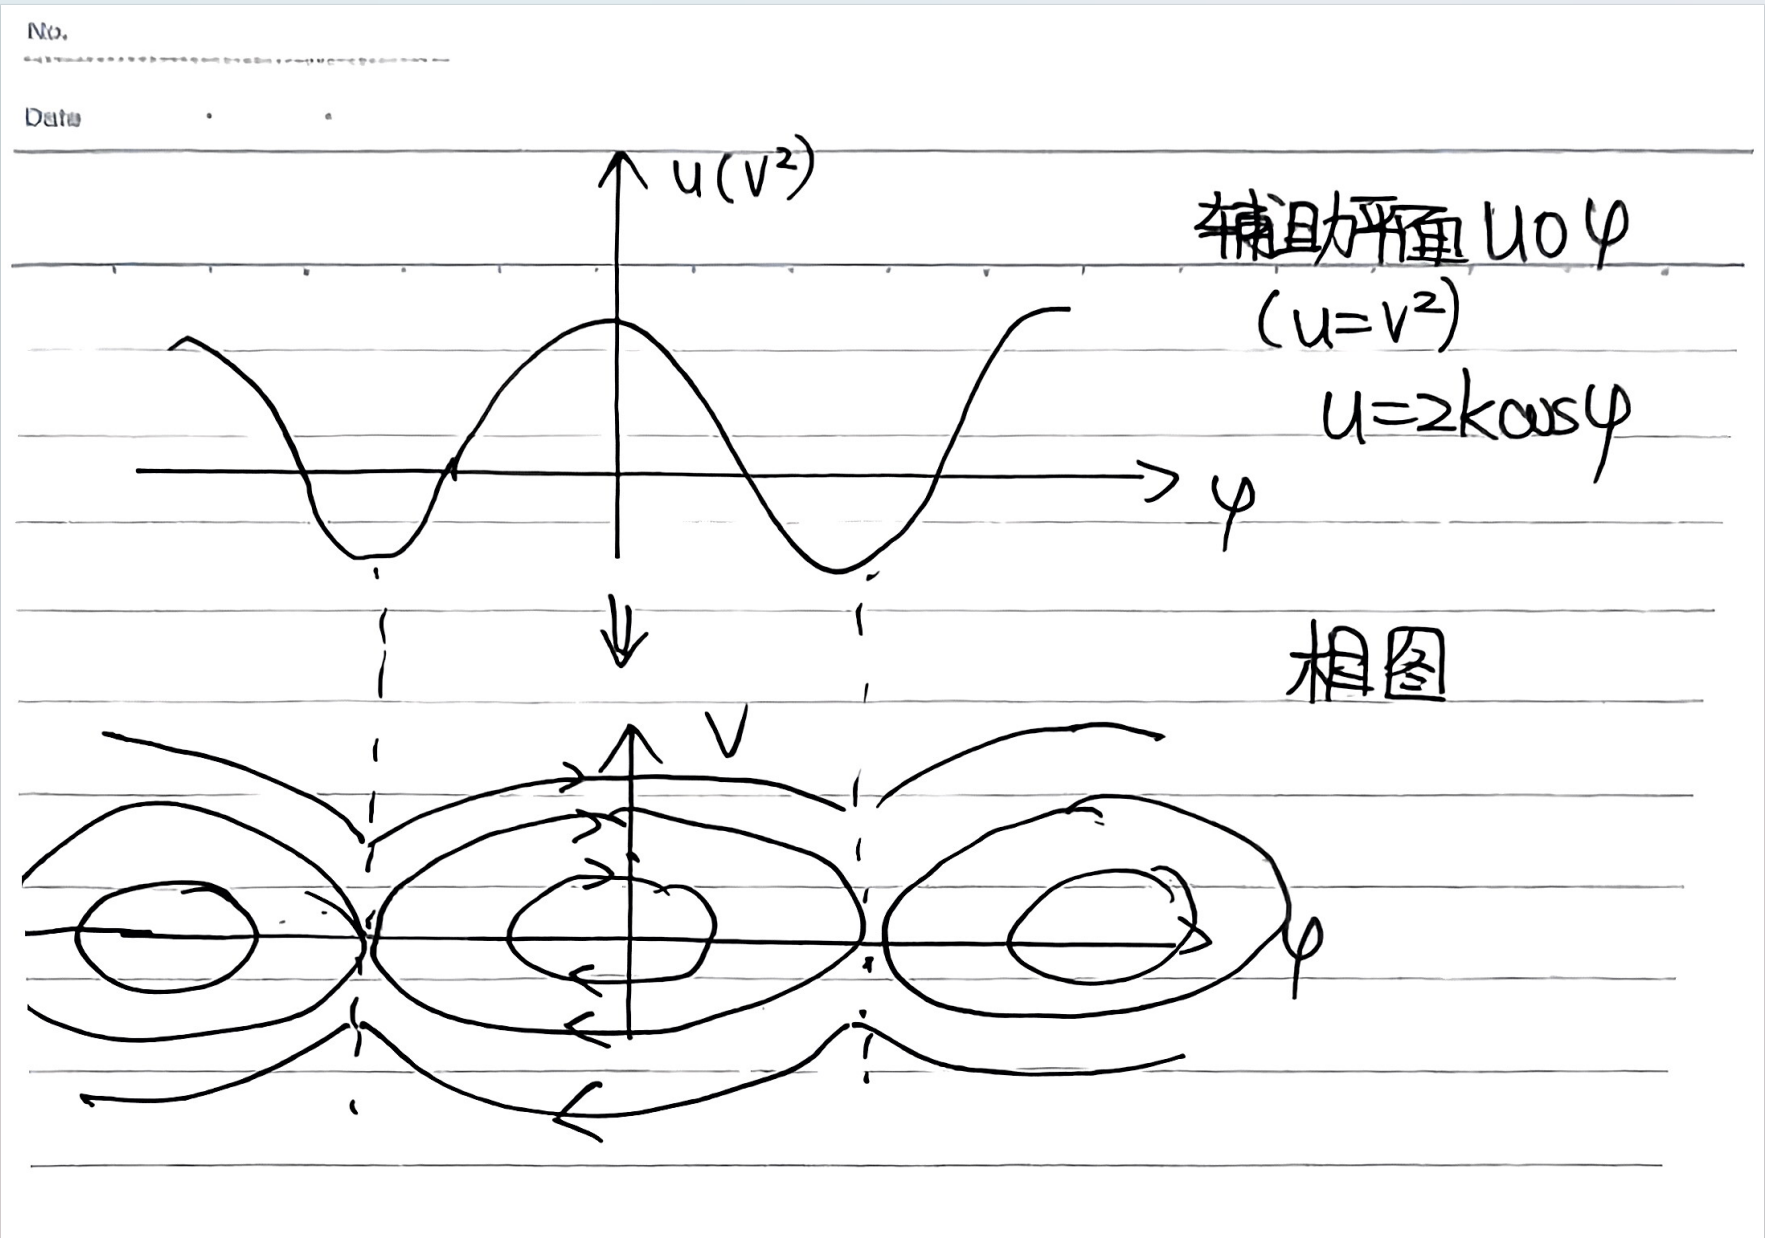
\includegraphics[height=5cm]{23期末.png} 
\label{fig:my_label}  
\end{figure}\\
(2)法一:(Lyapunov 函数)\\
取 $$V(x, y)=\frac{1}{2} y^{2}+\frac{g}{l}(1-\cos x) \quad$$\\ 满足 $V(0,0)=0$\\
$$\frac{d V}{d t}=\frac{\partial V}{\partial x} \cdot \dot{x}+\frac{\partial V}{\partial y} \cdot \dot{y}=\frac{g}{l} y \sin x-\frac{y}{l} y \sin x-\frac{\mu}{m} y^{2}$$\\
当无阻力时 $(\mu=0)$ :有 $\frac{d V}{d t} \equiv 0$ 故零解是稳定的\\
当有阻力时 $(\mu>0): ~ \frac{d V}{d t}$ 为常负(见书上定义)。由于满足 $\frac{d V}{d t}=0$ 的集合是 $y=0$ ,而在原点邻域中 $y=0$ 直线上除了零解 $x=0, y=0$之外不含有方程组的整条正半轨线,又由补充定理可以知道是渐近稳定的

\textbf{补充定理}:(王高雄 P270 定理5)\\
如果存在定正函数 $V(x)$ ,其通过方程组的全导数 $\frac{d v}{d t}$ 为常负。但使 $\frac{d v(x)}{d t}=0$ 的点 $x$ 的集合中除了零解外不包括方程组的整条正半轨线,则零解是渐近稳定的\\
法二:(线性近似)\\
将方程组写成 $$\left\{\begin{array}{l}\dot{x}=y \\ \dot{y}=-\frac{g}{l} x-\frac{\mu}{m} y-\frac{g}{l}(\sin x-x)\end{array}\right.$$\\
考虑线性近似方程组 $$\left\{\begin{array}{l}\dot{x}=y \\ \dot{y}=-\frac{g}{l} x-\frac{\mu}{m} y\end{array}\right.$$\\
非线性项:\\
$$
N(x, y)=-\frac{g}{l}(\sin x-x)=-\frac{g}{l}\left(-\frac{x^{3}}{3!}+\frac{x^{5}}{5!} \cdots\right)
$$
满足 $$N(t, 0)=0 ; \lim _{|(x, y)| \rightarrow 0} \frac{|N(x, y)|}{|(x, y)|}=0$$\\
考虑 \\$$A=\left(\begin{array}{cc}0 & 1 \\ -\frac{g}{l} & -\frac{\mu}{m}\end{array}\right)$$ \\特征值即可\\
特征值为 $$\lambda_{1,2}=-\frac{\mu}{2 m} \pm \frac{1}{2}\sqrt{\left(\frac{\mu}{m}\right)^{2}-4 \frac{g}{l}}$$
$\mu>0$ 时:特征值均有负实部,则零解渐近稳定\\
$\mu=0$ 时:特征值为纯虚数,无法判断非线性方程组是否稳定\\
五.\\
$$
\left\{\begin{array}{l}
\frac{d x}{d t}=x(2 y-1) \\
\frac{d y}{d t}=y(3-4 x)
\end{array}\right.
$$
且 $\varphi(t)=\binom{x(t)}{y(t)}$ 为方程周期为 $\omega$ 的解\\
求证:$$\quad \int_{0}^{\omega} \frac{\varphi(t)}{\omega} d t=\binom{\frac{3}{4}}{\frac{1}{2}}$$\\
证:先证 $$\int_{0}^{\omega} \frac{x(t)}{\omega} d t=\frac{3}{4}$$ \\
我们考虑将 $x(t)$ 降次为某个函数的导数\\
$\frac{d y}{d t}=y(3-4 x)$ 移项得到 $$\frac{d y}{y}=(3-4 x) d t$$ \\
$$\Rightarrow d(\ln |y|)=(3-4 x) d t$$\\
$$\Rightarrow x d t=\frac{3 d t-d(\ln |y|)}{4}$$\\
$$\Rightarrow \int_{0}^{\omega} x d t=\int_{0}^{\omega} \frac{3}{4} d t-\frac{1}{4} \int_{0}^{w} d(\ln |y|)$$\\
$$\Rightarrow \frac{3}{4} \omega - \frac{1}{4} \ln |y| \Big|_{w}^{0}$$\\
注意条件给出 $y(t)$ 周期为 $\omega \Rightarrow y(\omega)=y(0)$ 则 $$\int_{0}^{\omega} x d t=\frac{3}{4} \omega$$\\
另一边同理 $$\int_{0}^{\omega} y d t=\frac{1}{2} \omega$$\\
六.\\
考虑非齐次线性方程组
$$
x^{\prime}=A x+F(x)
$$
F 连续且 $\int_{x_{0}}^{+\infty}\|F(x)\| d x$ 有界,设其有基本解组 $\Phi(t)$\\
(1)求证:若$\|\Phi(t) \|$ 有界,则任意解在 $[0,+\infty]$ 有界\\
(2)求证:若 $\lim _{t \rightarrow+\infty}\|\Phi(t)\|=0$ 则任意解趋于$0$\\
证:\\(1)通解 $$x(t)=\Phi(t)\left(c+\int_{t_{0}}^{t} \Phi^{-1}(s) f(s) d s\right)$$\\
只需证 $\int_{t_{0}}^{t} \Phi^{-1}(s) f(s) d s$ 有界\\
又 $\Phi(t)$ 有界 $\Rightarrow$ 其元素有界 $\Rightarrow A_{i j}$ 有界且 $\operatorname{det}(\Phi)$ 有界且$\operatorname{det}(\Phi) \neq 0$\\
又 $$\Phi(t) \Phi^{*}(t)=\operatorname{det}(\Phi) I$$\\
$$\Rightarrow \Phi^{-1}(t)=\frac{\Phi^{*}(t)}{\operatorname{det}(\Phi)} \text{有界} M$$\\
$\int_{x_{0}}^{+\infty}\|F(x)\| d x$ 有界 $\Rightarrow \int_{t_{0}}^{t}\|F(x)\| d x$ 有界\\
则
 $$\int_{t_{0}}^{t} \Phi^{-1}(s) F(s) d s \leq M \int_{t_{0}}^{t} F(s) d s \quad \text{有界}$$\\
(2)仿照 1 证明 $\Phi^{-1}(t)$ 在 $t \rightarrow+\infty$ 有界即可


\end{document} 